\section{Software-Defined Networking}
\label{sec:background-sdn}

\begin{figure}[!ht]
    \centering
    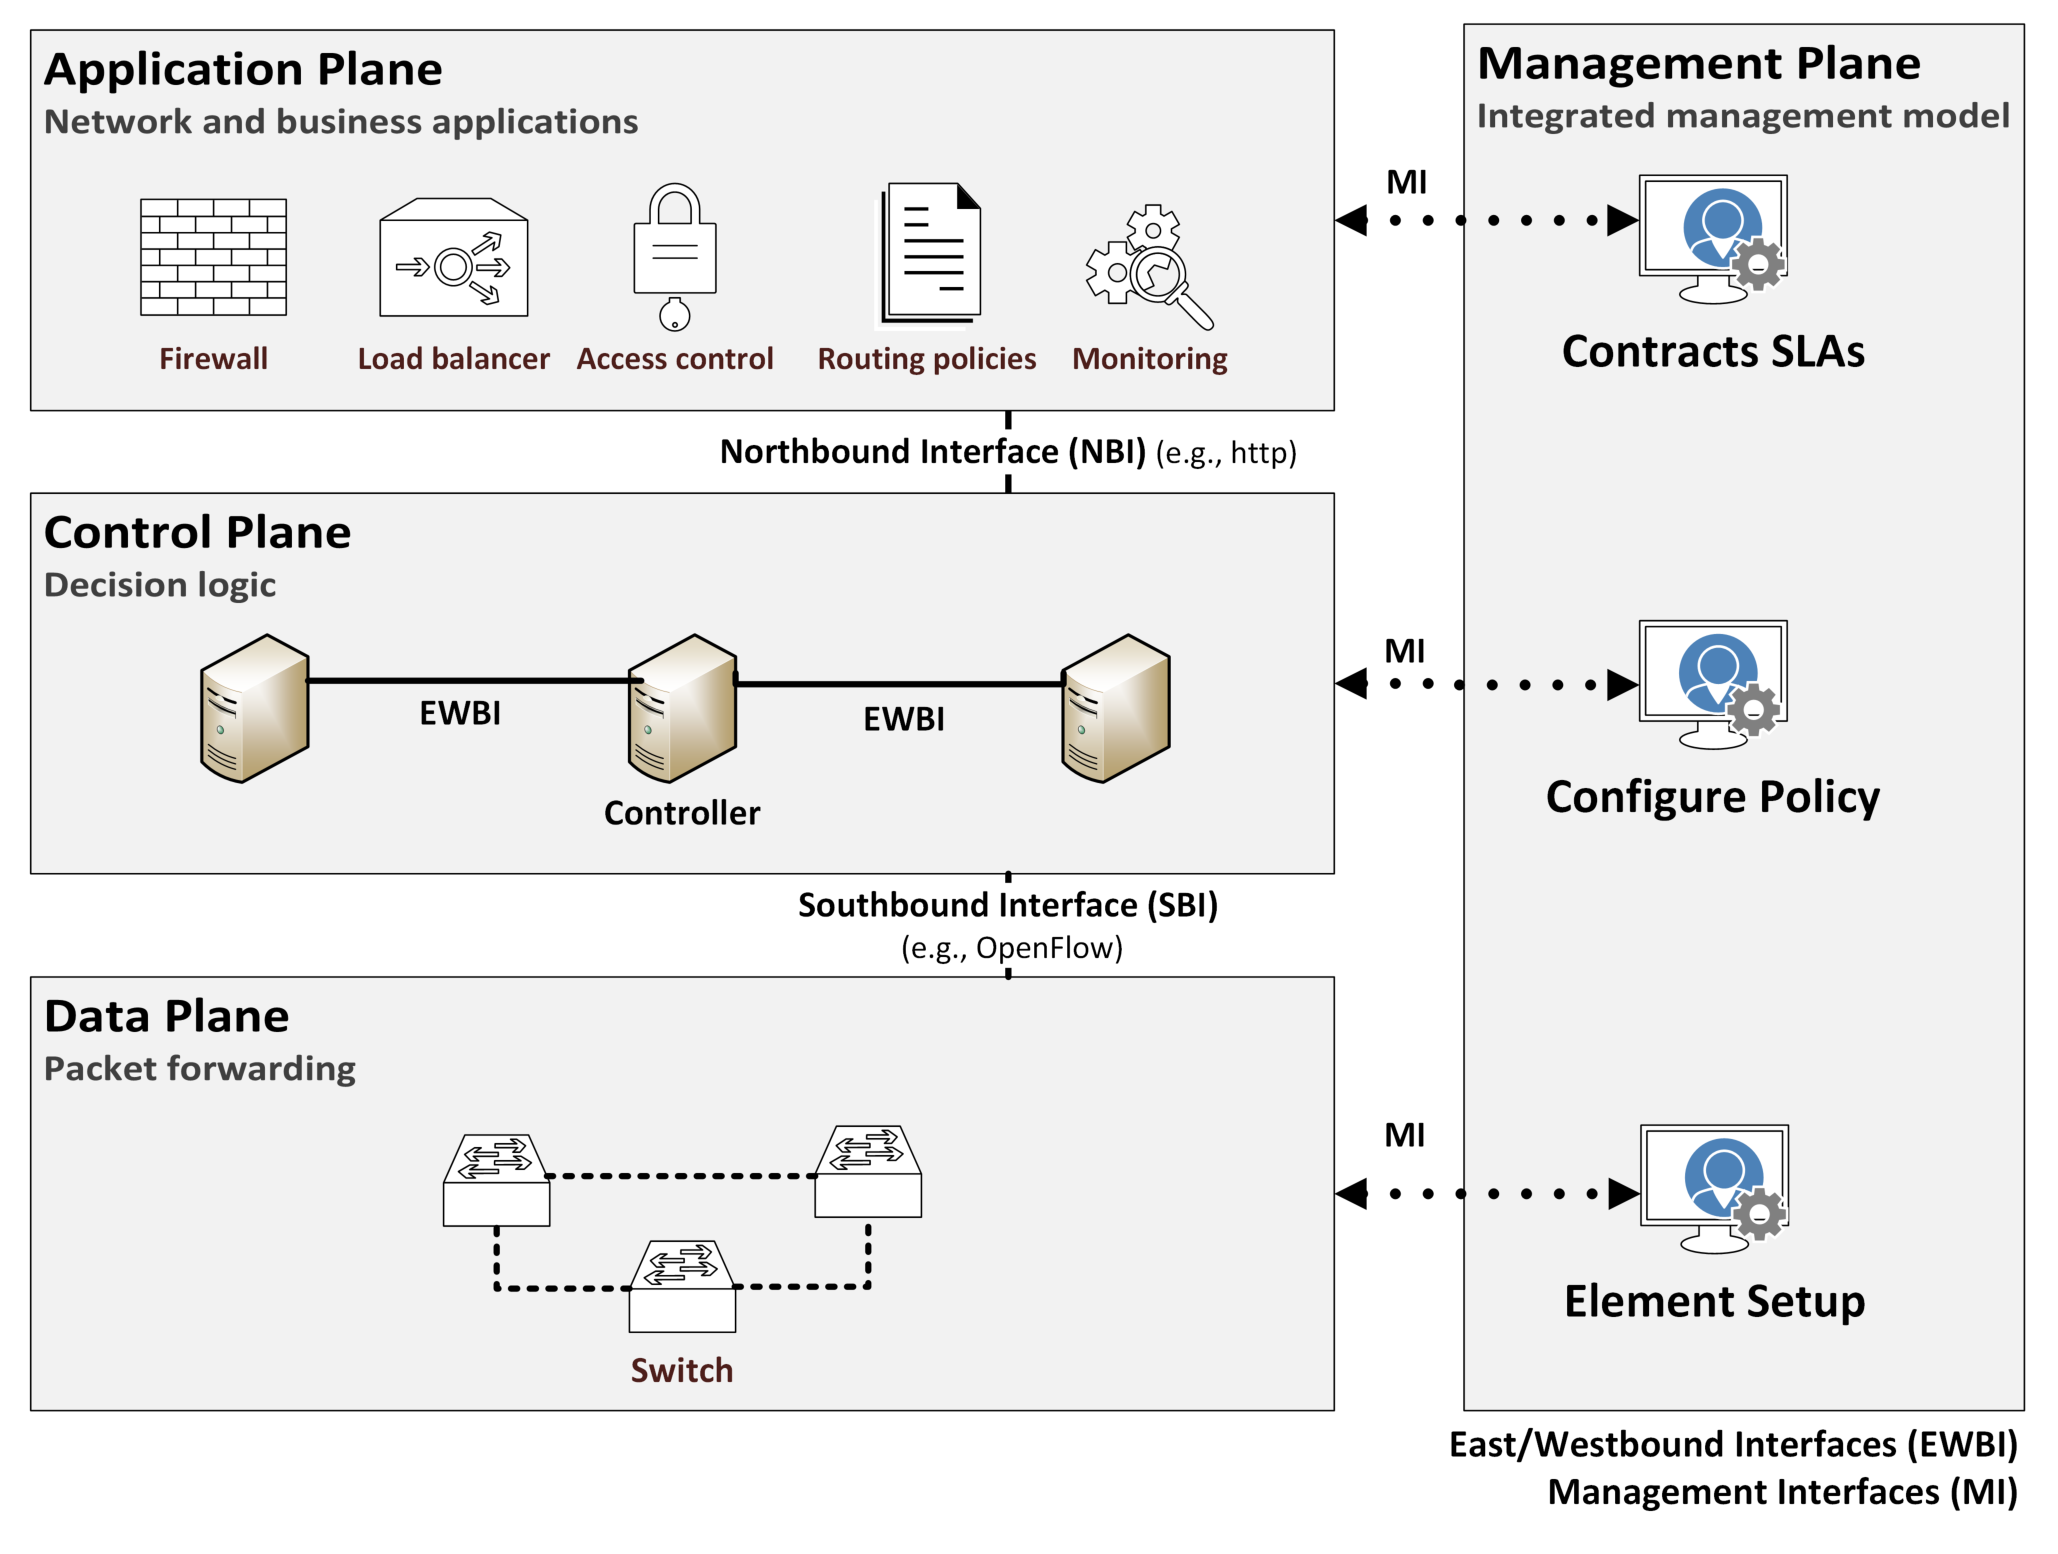
\includegraphics[scale=0.45]{figures/Figure_0_SDN_architecture}
    \caption{High-level SDN architecture}
    \label{fig:sdn_architecture}
\end{figure}

SDN represents one of the most well-known and attractive trends in academic and industry for defining the architecture of future networks \cite{ESTRADASOLANO2017150, feamster_2014:road_sdn}. SDN has some distinguishing features that define how it is different from traditional networking architecture. These features include \cite{kreutz_2015:sdn_comprehensive_survey, nunes_2014:survey_past_present_future}: (\textit{i}) clear separation of the control and forward function, (\textit{ii}) centralization of the control function, (\textit{iii}) implementation of the control function in software, (\textit{iv}) open standards, and (\textit{v}) Flow-based. These features make the SDN architecture more flexible, scalable, efficient and adaptable to the changing needs of the business \cite{herrera_2016:nfv_survey}. Furthermore, they make SDN a propitious scenario for efficiently and intelligently implementing monitoring techniques, particularly for TE.\\

Overall, SDN introduces an architecture with four planes \cite{onf_2014:sdn_architecture_overview}: management, application, control, and data (\textit{cf}. Figure~\ref{fig:sdn_architecture}). All these planes communicate with each other through interfaces. In particular, the Management Plane (MP) uses a set of Management Interfaces (MI) to exchange information and to control the other planes. The Application Plane (AP) communicates its network requirements to the Control Plane (CP) by NorthBound Interfaces (NBI). The CP defines East/Westbound Interfaces (EWBI) that enable to deploy a distributed controller for coping with large-scale and wide-area networks. The Data Plane (DP) communicates with CP by SouthBound Interfaces (SBI). Ideally,  all these interfaces should be standardized to allow easy replacement of devices and technologies. In practice, the OpenFlow protocol is the current \textit{de-facto} standard for the SBI because of its widespread use by vendors and research. All other interfaces are undergoing discussion and development.

\begin{itemize}
    \item \textbf{Management Plane} contains one or more solutions responsible for managing and coordinating each plane individually (\textit{e.g.}, network monitoring, performance management, configuring/planning resources, and enforcing both policies and contracts).
    
    \item \textbf{Application Plane} contains one or more applications that can serve different purposes (\textit{e.g.}, firewall, load balancer, access control, routing policies, and monitoring). Each application has access to a set of resources of one or more controllers through NBIs.
    
    \item \textbf{Control Plane} translates the requirements from AP at a specific network policy and enforces it over network elements through SBI. This plane contains one or more controllers (\textit{e.g.}, Floodlight, NOX, POX, and Ryu) that handle and coordinate the network devices.
    
    \item \textbf{Data Plane} contains a set of programmable network devices responsible for storing, forwarding and processing data packets. This plane depends on CP and MP to populate the forwarding tables and update their configuration.
\end{itemize}

%In \cite{onf_2013:sdn_architecture_overview}, the Open Networking Foundation (ONF) presents a high-level view of the SDN architecture along with its major components (Figure~\ref{fig:sdn_architecture}). At the bottom, the Data Plane (DP) is composed of network elements specialized in treating packages (forwarding), and it communicates with Control Plane (CP) by SouthBound Interfaces (SBI). The OpenFlow protocol \cite{mckeown_2008:openflow, kreutz_2015:sdn_comprehensive_survey, onf_2013:sdn_architecture_overview} is the most well-known open standard SBI because its widespread use by vendors and research. At the top, the Applications Plane (AP) implements and orchestrates the business logic and high-level networking functions (\textit{e.g.}, monitoring, routing policies, and access control). AP communicates its network requirements to the CP by NorthBound Interfaces (NBI). In the middle, CP translates application requirements and enforces them over network elements through SBI. CP also defines East/Westbound Interfaces (EWBI) that enable to deploy a distributed controller for coping with large-scale and wide-area networks. Furthermore, recent investigations have considered a Management Plane orthogonal to the whole SDN architecture for conducting integrated network management \cite{ESTRADASOLANO2017150}.

\section{Traffic Engineering}
\label{sec:background-te}

TE is emerging as an essential tool for selecting the optimal paths that different flows should follow to optimize resource utilization and satisfy the QoS requirements of each flow \cite{ian_2014:a_road_map_sdn, shu_2016:traffic_measurement_management}. According to the Internet Engineering Task Force (IETF), TE aims to evaluate and optimize network performance, QoS, and user experience of operational IP networks \cite{feamster_2014:road_sdn, awduche_2002:overview_ti, wang_2008:overview_routing_ti}. TE, in SDN, focuses on \cite{ian_2014:a_road_map_sdn}:

\begin{itemize}
    \item 
    \textbf{Flow Management (FM)} controls network resources appropriately when traffic congestion occurs in network nodes. FM maps and controls the traffic flow to steer traffic most efficiently. For example, when a switch receives flows that do not match any rule in the flows table; it forwards these flows to the controller. The controller analyzes this flow and decides to install it a new forwarding rule in the switches or to remove it. If the traffic consists of a high number of new flows or not match flows, it can generate a significant network overhead and latency at both CP and DP. FM looks for avoiding network overhead and providing a trade-off between load-balancing and latency.
    \item 
    \textbf{Fault Tolerance (FT)} seeks to ensure the immediate, transparent and graceful recovery of the network when a failure occurs in any of its nodes. FT provides mechanisms that enhance network integrity and adopts policies emphasising network survivable. For example, to increase the networking resiliency of SDN, FT could introduce a mechanism for link or node failures. This mechanism could specify alternative ports and paths that enable the switch to change the forwarding path in the policy-based routing without requiring a round trip to the controller.
    \item 
    \textbf{Topology Update (TU)} manages the capacity of the network to carry out planned changes (\textit{i.e.}, it aims to update the policies of the network in real time and ensure their application in each flow). For example, since the centralized controllers manage all switches, these can dynamically configure the global network policy rules. TU should guarantee consistency of the network policies across the switches so that each packet or flow should be handled by either the old policy or the new policy, but not by the two.
    \item 
    \textbf{Traffic Analysis/Characterization (TAC)} deals with the monitoring and verification of compliance with network performance goals to evaluate and debug the effectiveness of the applied TE methods. TAC focuses on mechanisms for monitoring the network, debugging errors, fault detection, data collection, and so on. In particular, TAC is the essential prerequisite for traffic analysis, and it is closely related to discovery the network failures and the prediction of link congestion.
\end{itemize}

An essential requirement for achieving TE is to provide accurate and reliable network monitoring (\textit{e.g.}, to perform TE \cite{al_2010:hedera}, it is necessary to correctly detect large flow aggregates in minutes and pick better routes for these flows). Many network management tasks such as traffic accounting, load balancing, and performance diagnosis all rely on accurate and timely monitoring of a large variety of traffic at different time-scales \cite{machado_2014:towards_SLA_Policy,tangari_2017:decentralized_monitoring,al_2010:hedera,benson_2011:microte}. 

\section{Network Monitoring}
\label{sec:background-ntm}

\subsection{Monitoring Operations}
\label{subsec:monitoring-operations}

Network Monitoring collects measurements of Key Performance Indicators (KPI) and events (\textit{e.g.}, bandwidth utilization and link status) to process them into more meaningful metrics, called Aggregate Metrics (\textit{e.g.}, average delay and network availability) \cite{mohan2011:active_passive}. Generally, network monitoring can be roughly classified into five phases: \textit{Collection, Preprocessing, Transmission, Analysis}, and \textit{Presentation} of the data \cite{tsai_2018:network_monitoring_review}. Figure~\ref{fig:monitoring_phases}, depicts the classification of operation phases in network monitoring.

\begin{figure}[!ht]
    \centering
    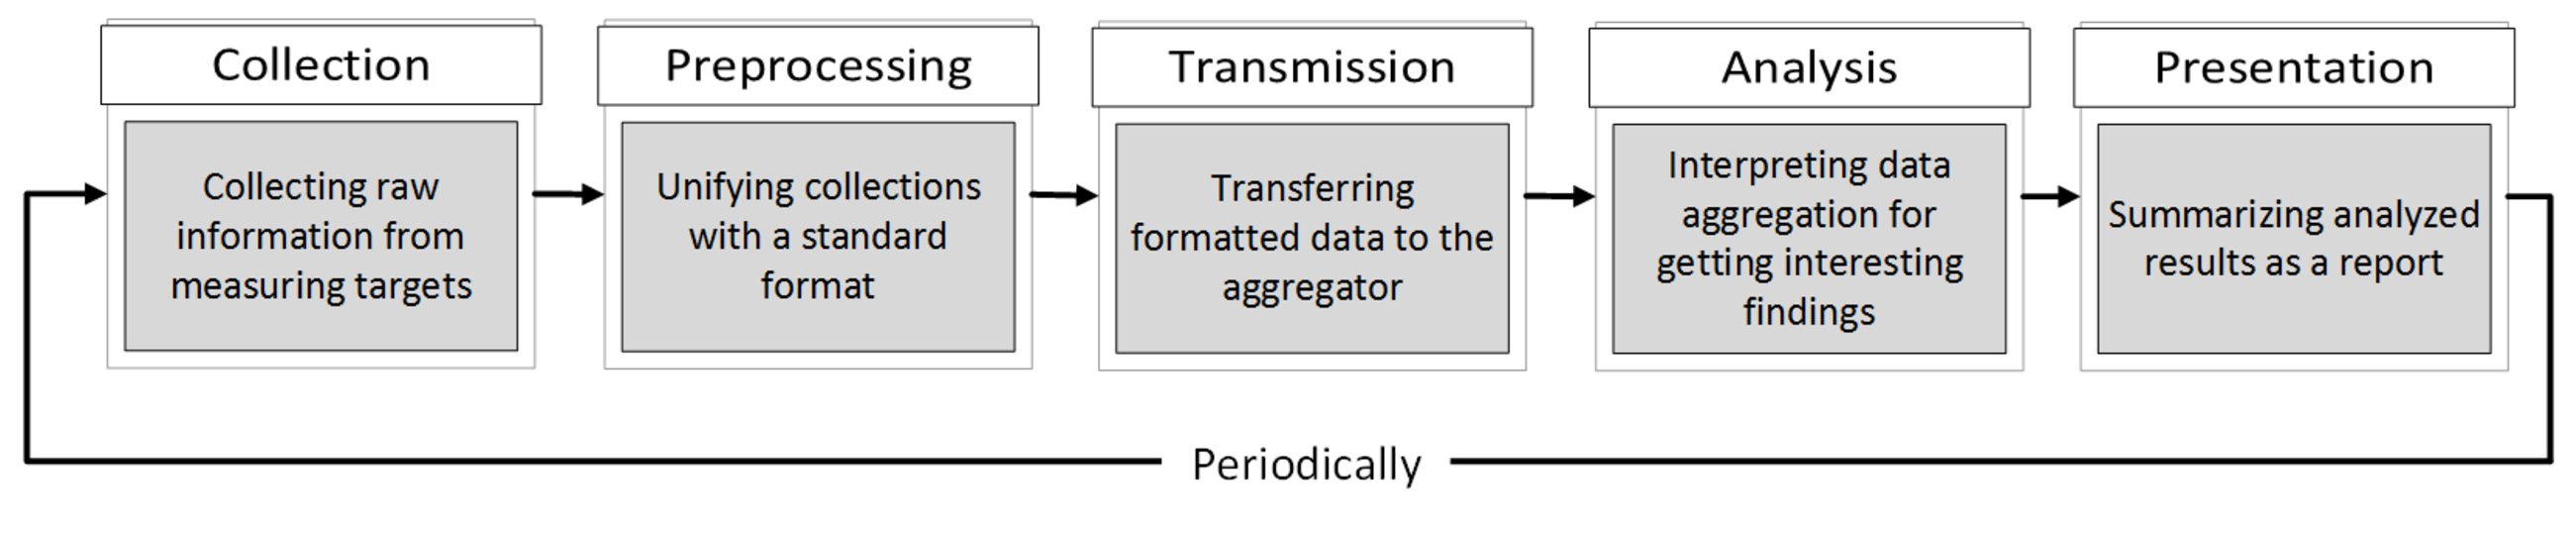
\includegraphics[scale=0.37]{figures/NetworMonitoringPhases}
    \caption{Classification of network monitoring operations (adapted from \cite{tsai_2018:network_monitoring_review})}
    \label{fig:monitoring_phases}
\end{figure}

\begin{itemize}
    \item \textit{Collection:} This phase raises three primary considerations namely, means, target, and probing interval. The means refers to how the data are to be collected. The target relates to the devices to be observed, and the probing interval indicates how often the data should be collected from switches.
    \item \textit{Preprocessing:} This phase is responsible for aggregating and turning the collected data into some statistical format. Furthermore, it helps to itemize and track the measurement results.
    \item \textit{Transmission:} This phase is responsible for carrying itemized data to the analytic station. The Simple Network Management Protocol (SNMP) and the Network Configuration Protocol (NETCONF) are typical protocols used to exchange messages in the transmission phase. These protocols provide a data delivery interaction between agents and the station.
    \item \textit{Analysis:} This phase generates statistics and identifies particular events. Some methods perform traffic analysis based on payload or host behavior, whereas other methods examine communication patterns \cite{Bujlow_2012:traffic_classificatiom_c5, dong_2012:traffic_clasification_ml}. The analysis results provide network status information to TE and fault management applications. 
    \item \textit{Presentation:} This phase exports the analysis results in tables, graphs, and reports. For example, Isolani \textit{et al.} \cite{isolani_2015:interactive} proposed an SDN Interactive Manager that provides data visualization via traffic graphs.
\end{itemize}{}

A critical task in network monitoring is to achieve a better performance in terms of low overhead (\textit{e.g.}, CCO and CUC) and high MA when measuring the network status. To achieve better performance, it is essential an accurate and timely collection of flow statistics \cite{rendon2014:monitoring}.

\subsection{Network Monitoring Techniques}
\label{subsec:monitoring-approaches}

In SDN, network monitoring techniques can be classified into two categories \cite{mohan2011:active_passive,Ningning_2003:probing_techniques}: push-based (called passive monitoring) and pull-based (called active monitoring). Although the focus of this dissertation is on the pull-based technique, both push-based and pull-based will be discussed briefly.

\begin{figure}[!ht]
        \centering
        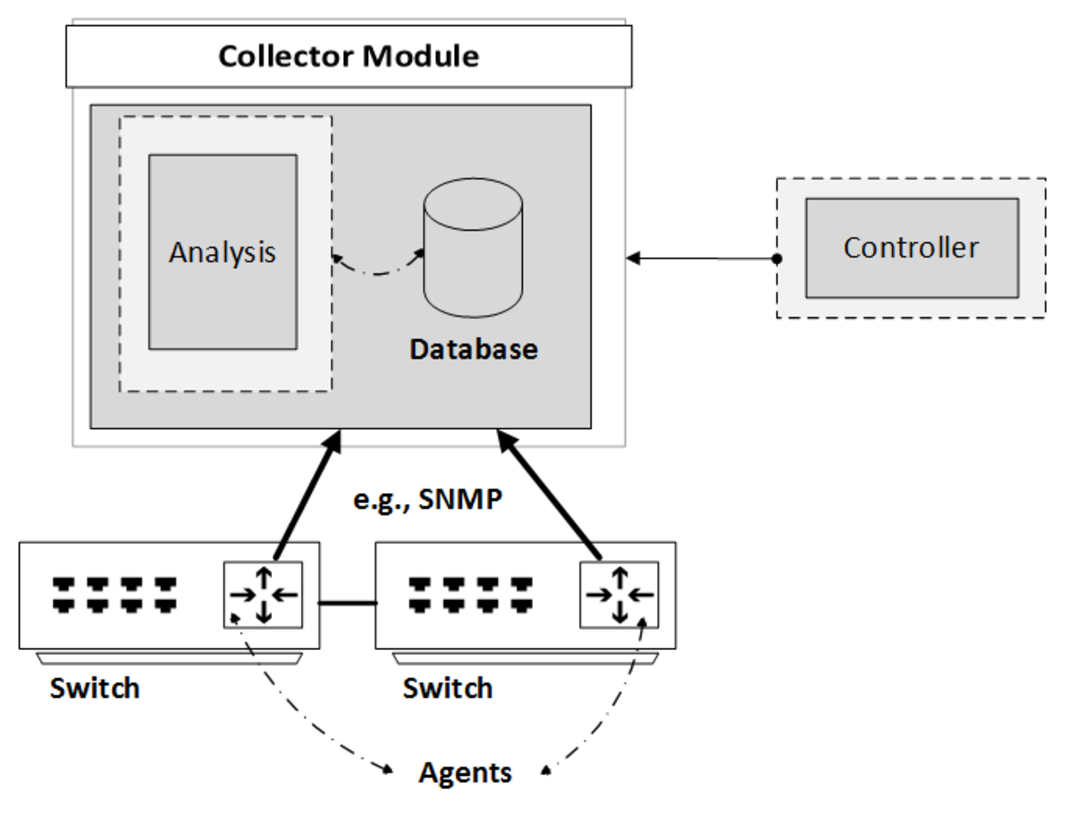
\includegraphics[scale=0.49]{figures/Push-Based}
        \caption{Push-based monitoring}
        \label{fig:push-based}
\end{figure}

\begin{itemize}
    \item In the \textbf{Push-based} approach \cite{claise2004:cisco_netflow,phaal2001:inmon_sflow}, the controller observes the statistics information supplied by a collector module without influencing in the performance of the network (\textit{cf.} Figure~\ref{fig:push-based}). In this approach, the statistical information is collected by agents placed inside switches (\textit{e.g.}, NetFlow \cite{claise_2004:cisco}, jFlow \cite{myers_1999:jflow}, sFlow \cite{wang_2004:sflow}), which observe and send the network traffic to the collector module using a monitoring protocol (\textit{e.g.}, SNMP and NETCONF). The collector module is responsible for analyzing and storing this network traffic to make it available to the controller.
    
    Although Push-based approach does not intervene in the performance of the network, several factors hinder its applicability. First, additional elements are necessary in the hardware and software of switches. Second, when the traffic varies dynamically, switches frequently detect no-matching packets in the flow table and, as a result, massive statistical reports are sent to the controller. These massive reports can cause significant CCO \cite{aslan_2016:impact} and CUC \cite{su_2014:flowcover}. Third, the push-based approach requires full access to network devices, which could raise privacy and security issues.
    
    %\item \textbf{Pull-based} injects test packages (\textit{e.g.}, ping and traceroutes) into the network for measuring the response and checking the result for important metrics such as latency, jitter, throughput, and packet loss. 
    \item In the \textbf{Pull-based} approach, the controller probes one, a set, or all switches using Read-State messages to retrieve statistics from switches (\textit{cf.} Figure~\ref{fig:pull-based}). There are two variations of Read-State messages: \textit{Request} and \textit{Reply}. The  \textit{Request} messages are sent from the controller to switches to request the specific statistical information. The \textit{Reply} messages, on the other hand, are sent from the switches to the controller, delivering the required statistical information.
    
    \begin{figure}[!ht]
        \centering
        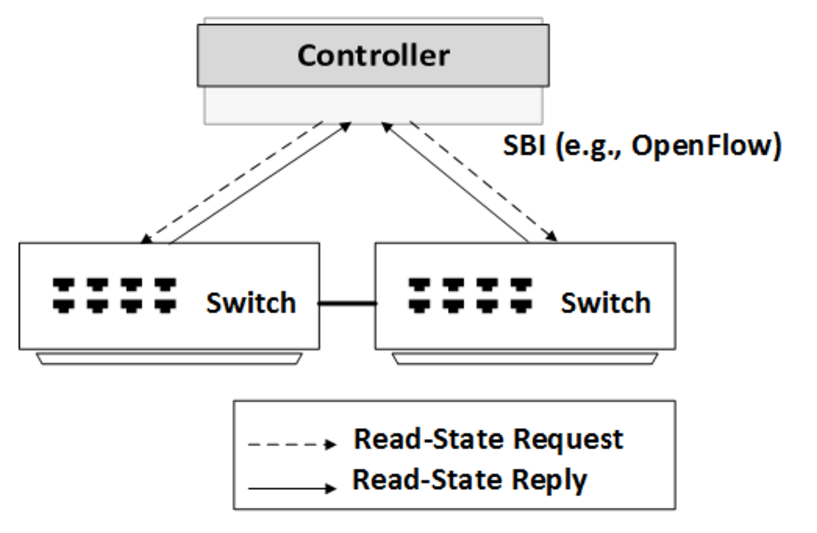
\includegraphics[scale=0.6]{figures/Pull-Based}
        \caption{Pull-based monitoring}
        \label{fig:pull-based}
    \end{figure}
       
    This approach provides flexibility, since it can asynchronously communicate with switches to request the specific state information and control the size of statistical reports. Nonetheless, CCO can also be introduced in the pull-based approach because of the probing interval. This overhead can lead to overload the controller (\textit{i.e.}, increase CUC) and significantly interfere with essential SDN functions, such as packet forwarding and route updating \cite{Malboubi_2015:SNIPER}.
\end{itemize}

This master dissertation focuses on the pull-based approach because:
\begin{itemize}
    \item It allows requesting specific statistical information from one, a set, or all switches asynchronously, allowing the controller to collect statistical information flexibly and control the size of statistical reports.
    \item It does not require changes in the software and hardware of switches because the controller only needs Read-State messages, intrinsic in SDN switches, to retrieve statistical information.
\end{itemize}

\section{Machine Learning}
\label{sec:background-ml}

The quantity of data that flows through communication networks is increasing exponentially. The extraction of knowledge from this data is becoming increasingly important to perform efficient monitoring and management of the network. ML is a tool used to extract useful knowledge from the data and make appropriate decisions \cite{sara_2018:ml_cognitive_network_management,Mowei_2017:ml_Workflow,stampa_2017:DL_optimization}.\\

ML includes a set of techniques that can automatically detect patterns in the data (patterns that do not conform to the normal network behavior) to identify previously unseen events and thus to detect network anomalies and to predict future data \cite{murphy_2012:ml_probabilistic,bishop_2006:pattern_recognition}. The possibilities that emerge from the use of ML in networking context are various \cite{Boutaba2018}, some examples are:

\begin{itemize}
    \item \textit{Network traffic prediction:}  Li \textit{et al.} \cite{li2016predicting} proposed an ML technique that focus is on predicting incoming and outgoing traffic volume on an inter-data center link dominated by elephant flows. Poupart \textit{et al.} \cite{Poupart_2016:online} explored the use of ML for flow size prediction and elephant flow detection. Chen \textit{et al.} \cite{chen2016predicting} investigated the possibility of reducing the cost of monitoring and collecting traffic volume, by inferring future traffic volume based on flow count only.  %\cite{sun_2016:cs2p}.,chen_2016_predicting_traffic}.
    
    \item \textit{Resource management:} Bojovic \textit{et al.} \cite{bojovic2012cognitive} designed an ML-based radio admission control mechanism to guarantee QoS for various services, such as voice, data, video and FTP while maximizing radio resource utilization in long term evolution (LTE) networks. Vassis \textit{et al.} \cite{vassis2014admission} proposed an adaptive and distributed admission control mechanism for variable bitrate video sessions, over ad hoc networks with heterogeneous video and HTTP traffic. Quer \textit{et al.} \cite{quer2011cognitive} developed an admission control mechanism for VoIP calls in a WLAN. They employed ML to predict the voice call quality as a function of link-layer conditions in the network.
    
    \item \textit{Fault management:} Snow \textit{et al.} \cite{snow2005assessing} used ML to estimate the dependability of a 2G wireless network, which is used to characterize availability, reliability, maintainability, and survivability of the network. Lu \textit{et al.} \cite{lu2009using} use a manifold learning technique to automatically extract failure features and generate failure prediction. Pellegrini \textit{et al.} \cite{pellegrini2015machine} proposed an ML-based framework to predict the remaining time to failure of applications.
    
    \item \textit{Congestion control:} Liu \textit{et al.} \cite{liu2003end} proposed an approach using ML for inferring the cause of packet loss in hybrid wired-wireless networks. Fonseca and Crovella \cite{fonseca2005bayesian} focused on detecting the presence of packet loss by differentiating Duplicated ACKs caused by congestion losses and reordering events. Jayaraj \textit{et al.} \cite{jayaraj2008loss} tackled the classification of congestion losses and contention losses in optical burst switching networks.% \cite{dong_2015:pcc}.
\end{itemize}{}

Furthermore, ML has been used successfully in other domains, including agriculture \cite{efcastillo_2016:agriculture, efcastillo_2015:agriculture, ZHANG_2005:agriculture}, economics \cite{kim_2004:usefulness, nielsen_2004:local}, and cybersecurity \cite{Dua_2011:DM_ML_Cybersecurity, Thuraisingham_2003:ciber}.\\

ML can be divided into three categories, based on how the learning is achieved \cite{ayodele_2010:introduction, bishop_2006:pattern_recognition}:

\begin{itemize}
    \item \textbf{Supervised Learning (SL)} requires a set of instances, commonly known as training data, which are used to define the behavior of algorithm. The training data consists of a set of attributes and an objective variable (also called class), which is intended to be classified or predicted. When the domain of the attribute is categorical\footnote{A domain is defined as categorical if it is finite (discrete numerical values) and unordered}, the problem is known as classification or pattern recognition, and when the domain of the attribute is numeric\footnote{A numeric domain consists of real numbers} value, the problem is known as regression. The most representative algorithms of SL are: Bayesian Networks, Support Vector Machines, k-Nearest Neighbors, Decision Trees, and Neural Networks \cite{Mowei_2017:ml_Workflow,Boutaba2018}.
    
    \item \textbf{Unsupervised Learning (UL)} explores the structure of a non-tagged dataset (without target variable). This method reveals unexpected characteristics (patterns) and generates new groups (each with different identifiable properties). The unsupervised learning algorithms are divided into three relevant categories: 
    
    \begin{itemize}
        \item \textit{Hierarchical Algorithm} aims to obtain a hierarchy of clusters, called dendrogram, that shows how the clusters are related to each other \cite{Grira_2004:ml_techniques}.
        
        \item \textit{Density Algorithm} finds the areas with the highest data density, leaving aside the sparsely populated regions, which are considered border points or noise \cite{rehman_2006:density_based_clustering}.
        
        \item \textit{Clustering Partitional Algorithms} aims to directly obtain a single partition of the collection of items into clusters \cite{Grira_2004:ml_techniques}.
    \end{itemize}{}
    
    \item \textbf{Reinforcement Learning (RL)} is an iterative process in which an agent learns a decision-making process by interacting with the environment (\textit{cf.} Figure~\ref{fig:rl}). The agent is aware of the state of the environment and takes actions that produce changes of state. For each action, the agent receives a reward depending on how good was the action taken. The goal of the agent is to maximize the total reward it receives over time.
    
    \begin{figure}[!ht]
        \centering
        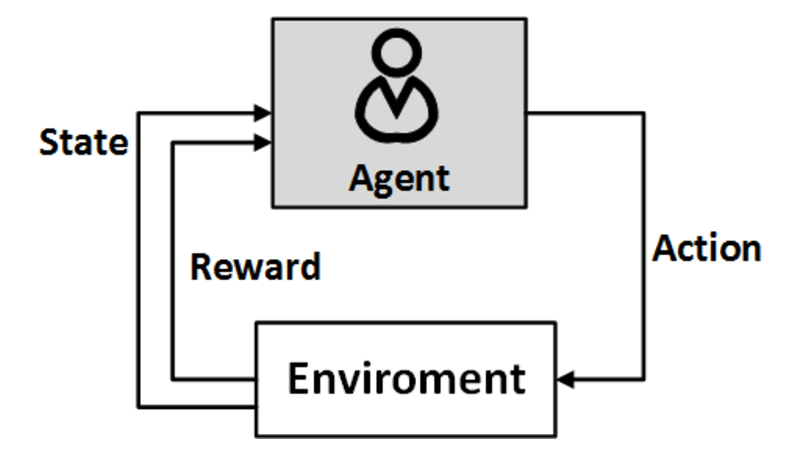
\includegraphics[scale=0.6]{figures/rl}
        \caption{RL Process}
        \label{fig:rl}
    \end{figure}
    
    RL is best suited for making cognitive choices, such as decision making, planning, and scheduling. For instance, RL has been successfully applied to complex problems such as board games \cite{tesauro_1995:temporal}, job-shop scheduling \cite{yoshimoto_1999:application}, elevator dispatching \cite{crites_1998:elevator}, and motor control tasks \cite{doya_2000:reinforcement}, either simulated or real \cite{schaal_1994:robot}.
    
\end{itemize}